\documentclass[report]{subfiles}
\begin{document}
    \chapter{IMPLEMENTATION}
    The source code for this project can be accessed through the GitHub repository of the project:\\
    \url{https://github.com/Sem-Projects/logic-simulator-inator}
    \section{Brief Description of the Files}
    The source code for our project has been divided into 9 files which consists of 5 C source files and 4 header files. They have been briefly explained below.
    \subsection{component.c \& component.h}
    As the name suggests, these files contain all the necessary information about the components used in the program. The header file defines a structure named Component that encompasses the details about a component including its size, position, input source, number of inputs, input state(s), output state(s) and other information which is later used.
    The output of any component (except clock and state) depends on its input(s). To get the desired output for any component from its inputs, the source file defines different component specific functions. The working of these functions is pretty straight-forward as they follow the standard logic operations available in C. As for the clock, its output is generated based on the value of time variable, which changes as the program progresses, defined in program.c. The clock inverts its current state when time reaches a certain value. The output of state is inverted when the user clicks on it.
    \subsection{draw.h \& draw.c}
    These two files contain the variables and functions that are responsible for drawing all the elements that are visible on the screen such as Buttons, Components, and Wires. It also handles rendering text in the SDL window where necessary. The header file defines an enumeration of confirmation flags that are later used to ask the user for confirmation on certain operations.
    The standard rendering functions available in the SDL library are used in order to draw Buttons and Components. However, SDL does not offer the functionality to draw curves. So, a simple algorithm that approximates a cubic Bezier Curve is used to draw wires.
    As for displaying text, a character map consisting of all the ASCII characters is predefined when the program starts. The font used is robotoo.ttf. The character map is later used to display any text (ASCII based) on the screen.
    \subsection{interaction.h \& interaction.c}
    User interaction is an integral part of any program, even more so for programs that use both mouse and keyboard to take input. These two files are responsible for handling such interactions. The header file defines various structures that are necessary for the Undo/Redo functionalities.
    The source file defines different functions that determine what will happen when a certain button is pressed or when a component is placed on the grid. Since these functions handle interaction with the user, they are usually only called when an event occurs. An SDL event encompasses mouse clicks, keyboard presses, etc. Different functions are called for different events. This coordination is handled in the file program.c.
    \subsection{program.h \& program.c}
    To keep the main.c file clean, the main program loop is defined in this file. For this reason, it acts as the centerpiece of the program that coordinates the functions of all other files. To begin with, the header file defines macros for configuring the main window and different elements inside it. Also, the colors that are frequently used in the program are defined here.
    The source file can be vaguely divided into two parts: Initialization and Main Program Loop. The initialization part is responsible for setting up all the necessary elements needed for the program to function properly. This is a one-time process that occurs when the program is launched.
    The Main Program Loop, as the name suggests, is a loop that runs over and over until the user exits the program. Everything that the user does inside the program is handled in this section. During each loop, the program checks for events, performs necessary operations based on them, updates the elements on the screen if required, and redraws all of those elements.
    \subsection{main.c}
    As mentioned earlier, this file is kept as clean as possible by defining the main loop in program.c. Inside this file, the current working directory is changed to the folder containing the executable and font files, so that the font files are always found regardless of where the program is run from. This is done using the <direct.h> library.
    The main function calls functions for initialization, the main program loop, and finally closing the program.
    \section{Rendering}
    \textit{Note: Throughout this document, the words rendering and drawing have been used interchangeably}\\
    There are generally two ways to display graphic elements in an SDL window - displaying images using SDL surfaces or hardware rendering with textures and renderer. This program uses the later as the elements are too versatile to store them as bitmaps.
    \begin{figure}[H]
        \centering
        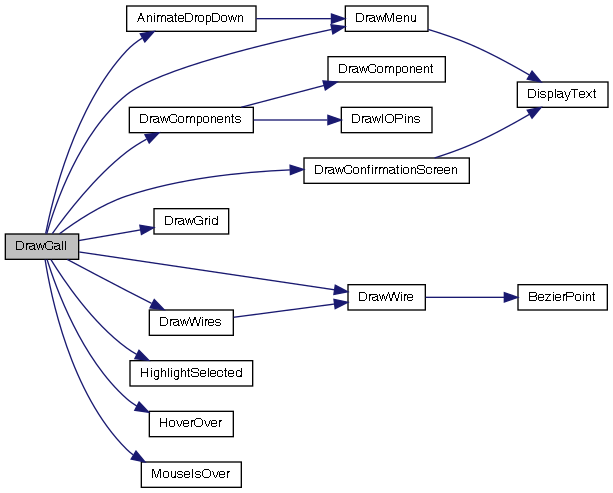
\includegraphics[width=0.5\textwidth]{graphics/render_call_tree.png}
        \caption{Call tree for Rendering}
    \end{figure}
    For rendering all elements of the program, many functions have been called as shown in above figure. Most of these functions have been described below.
    \subsection{Functions for rendering in SDL}
    SDL provides a handful of functions which can be used to draw shapes such as lines, points, rectangles and filled rectangles. These shapes are very simple however the can be utilized to draw other complex shapes. But before we render a shape, we have to set its color.
    Each element on the screen may have a different color. So the renderer stores the color information when drawing anything on the screen. This information is stored if 4 channels commonly known as rgba format. The first three channels indicate intensity of red, green, and blue color respectively. The last channel is used to store the opaqueness of the element. The higher the value the higher the intensity. Before drawing an element on the screen, we must make sure that the renderer is set to the correct color value. This can be done using the function shown below.
\begin{lstlisting}
// SDL_SetRenderDrawColor(SDL_Renderer *, int red, green, blue, alpha);
SDL_SetRenderDrawColor(renderer, 255, 255, 255, 255);     //opaque white color
\end{lstlisting}
    \textbf{Rendering Lines}\\
    As mentioned previously, SDL provides direct functionality to draw a straight line between two points. The data doesn't need to be stored anywhere instead we can simply pass the co-ordinates of the points as parameters to the \texttt{SDL\_RenderDrawLine()} function and it will draw a line between those points for us. The co-ordinates are relative to the top left point of the window. This function has been used to draw the grid lines.
\begin{lstlisting}	
// SDL_RenderDrawLine(SDL_Renderer *, startX, startY, endX, endY);
SDL_SetRenderDrawLine(renderer, 0, 0, 50, 50);            //diagonal line form top left corner
\end{lstlisting}
To draw many lines at once, the \texttt{SDL\_RenderDrawLines()} function can be used which which takes an array of \texttt{SDL\_Point} and draws may lines by joining $n^{th}$ point in the array to the $(n + 1)^{th}$ point. This function has been used to draw wires joining the components.
\begin{lstlisting}	
SDL_RenderDrawLines(SDL_Renderer *, SDL_Point *array_of_points, int no_of_points);
\end{lstlisting}
    \textbf{Rendering Rectangles}\\
    In exchange for the low level access SDL provides, a lot of abstraction has been taken away. A rectangle is arguably the most complicated shape that can be drawn directly from the renderer in SDL. It can either be a rectangular outline or a solid rectangle filled with the current color configurations. In order to do so, the data for a rectangle must be stored using \texttt{SDL\_Rect} structure.
    \texttt{SDL\_Rect} structure has following members:
\begin{lstlisting}
    int x, y;    // coordinate of top left corner of the rectangle
    int w, h;    // width and height of the rectangle
\end{lstlisting}
The \texttt{SDL\_RenderDrawRect()} function can be used to render an outline of a rectangle and \texttt{SDL\_RenderFillRect()} function can be used to render a filled rectangle. Both of these functions take a \texttt{SDL\_Renderer *} and a \texttt{SDL\_Rect *} as parameters.
\begin{lstlisting}
SDL_Rect example = {10, 10, 200, 400};
SDL_SetRenderDrawColor(renderer, 255, 0, 0, 255);
//SDL_RenderDrawRect (SDL_Renderer *, SDL_Rect *);
SDL_RenderDrawRect (renderer, &example); // draws a red outline of a 200x400 px rectangle whose top left corner is at 10, 10
//SDL_RenderFillRect (SDL_Renderer *, SDL_Rect *);
SDL_RenderFillRect (renderer, &example); // draws a filled red 200x400 px rectangle whose top left corner is at 10, 10
\end{lstlisting}
The \texttt{SDL\_RenderDrawRect()} function has been used to draw highlight border around buttons and components. The \texttt{SDL\_FillRect()} has been heavily used to draw buttons, components, dialog boxes and menus.\\
In addition to these, \texttt{SDL\_RenderFillRects()} and \texttt{SDL\_RenderDrawRects()} are also available which can be used to draw multiple rectangles at once. We have used these functions to draw input/output terminals for the components.
\begin{lstlisting}	
SDL_RenderDrawRects(SDL_Renderer *, SDL_Rect *array_of_rect, int no_of_rects);
SDL_RenderFillRects(SDL_Renderer *, SDL_Rect *array_of_rect, int no_of_rects);
\end{lstlisting}
% 	\begin{figure}[H]
%     \centering
%     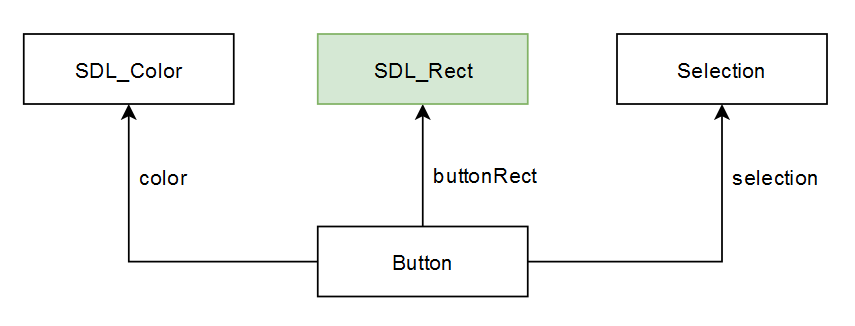
\includegraphics[width=0.8\textwidth]{graphics/button_structure.png}
%     \caption{Button Structure}
% 	\end{figure}
% The structure for Button contains a buttonRect element which stores the position and size information for that button. Later, it is used to draw the rectangle as follows:
% \begin{lstlisting}
% //SDL_RenderFillRect (renderer, &rectangle);
% SDL_SetRenderDrawColor (renderer, &Run.buttonRect);            //the rectangle for the Run button
% \end{lstlisting}
    \textbf{Rendering Text}\\
    As mentioned earlier, the text rendering is handled by an extension of the SDL library - SDL\_ttf. It provides the functionality to load ttf, rtf or otf fonts and create textures from them. An array of texture pointers is used to store the necessary ASCII characters. A texture is a structure that stores pixel data that can only be accessed through the GPU. Later, this array is used to display any message we want.
    In our program, we have implemented the text rendering as follows:\\
    \begin{lstlisting}
// First, fonts are initialized
TTF_Font *font = NULL;             //Font used in UI
TTF_Font *displayFont = NULL;      //Font used in decoders
static void InitFont(){
    TTF_Init();     // Initialize SDL_ttf
    // open fonts
    font = TTF_OpenFont("ui_font.ttf", 25);
    displayFont = TTF_OpenFont("led_font.otf", 100);
    // check if fonts were found
    if (font == NULL || displayFont == NULL){
        SDL_Log("Failed to load the font: %s\n", TTF_GetError());
        exit(-3);
    }
}

// Then, character maps are created
SDL_Texture *characters[127 - 32]; //Character map for UI
int characterWidth[127 - 32];  // Width of characters (to maintain proper shape of characters)
SDL_Texture *displayChars[16]; // Character Map for decoders
void CharacterMap(){
    // character to be displayed on decoders
    char *nums[16] = {"0", "1", "2", "3", "4", "5", "6", "7", "8", "9", "A", "B", "C", "D", "E", "F"};
    SDL_Surface *characterSurface; // surface which will be used to create texture
    SDL_Color white = {WHITE, 200};
    SDL_Color black = {BLACK, 255};
    // create textures for characters having ASCII value 32 - 127 (all required characters)
    for (int i = 32; i < 127; i++){
        // render character on surface
        characterSurface = TTF_RenderText_Blended(font, (char *)&i, white);  
        // create texture from surface and store in array
        characters[i - 32] = SDL_CreateTextureFromSurface(renderer, characterSurface);
        // get width of surface and store in array
        characterWidth[i - 32] = characterSurface ? characterSurface->w : 0;
    }
    // create textures for characters in nums array
    for (int i = 0; i < 16; i++){
        characterSurface = TTF_RenderText_Blended(displayFont, nums[i], black);
        displayChars[i] = SDL_CreateTextureFromSurface(renderer, characterSurface);
    }
    SDL_FreeSurface(characterSurface);
}

// render the text
static void DisplayText(char *message, SDL_Rect parent){
    char *tmp = message;
    int totalWidth = 0; // total width of the message in pixels 
    float factor = 1; // factor to resize the text if it is too long
    // calculate total width
    for (; *tmp; tmp++)
        totalWidth += characterWidth[*tmp - 32];
    // rect onto which text will be rendered
    SDL_Rect charDest = {.y = parent.y, .h = parent.h};
    // calculate the factor
    if (totalWidth > parent.w){
        factor = parent.w / (float)totalWidth;
        tmp = message;
        totalWidth = 0;
        for (; *tmp; tmp++)
            totalWidth += characterWidth[*tmp - 32] * factor;
    }
    // center the text relative to the parent rect
    charDest.x = parent.x + (parent.w - totalWidth) / 2;
    // render each character in message onto the screen
    for (int i = 0; *message; message++, i++){
        charDest.w = characterWidth[*message - 32] * factor;
        SDL_RenderCopy(renderer, characters[*message - 32], NULL, &charDest);
        charDest.x += charDest.w;
    }
}
    \end{lstlisting}
	\subsection{Drawing the Menu}
\begin{lstlisting}
static void DrawMenu(bool menuExpanded, bool simulating, bool snap, Selection choice){
    // width, height of the window
    int w, h;
    SDL_GetWindowSize(window, &w, &h); 
    // background of menu
    SDL_Rect menuBg = {0, 0, MENU_WIDTH, h};
    SDL_SetRenderDrawColor(renderer, BG1); 
    SDL_RenderFillRect(renderer, &menuBg);
    // draw RUN/STOP button
    SDL_SetRenderDrawColor(renderer, SideMenu[sm_run].color.r, SideMenu[sm_run].color.g, SideMenu[sm_run].color.b, 255);
    SDL_RenderFillRect(renderer, &SideMenu[sm_run].buttonRect);
    if (simulating)
        DisplayText("STOP", SideMenu[sm_run].buttonRect);
    else
        DisplayText("RUN", SideMenu[sm_run].buttonRect);

    //draw all buttons in the side menu
    SDL_SetRenderDrawColor(renderer, SideMenu[sm_compo].color.r,  SideMenu[sm_compo].color.g, SideMenu[sm_compo].color.b, 255);
    for (int i = 1; i < sm_total; i++){
        if (i == sm_inc || i == sm_dec && choice.type < g_and)
            continue;
        SDL_RenderFillRect(renderer, &SideMenu[i].buttonRect);
        DisplayText(SideMenuButtonText[i], SideMenu[i].buttonRect);
    }

    if (snap)
        DisplayText("Snap to Grid: On", SideMenu[sm_snap].buttonRect);
    else
        DisplayText("Snap to Grid: Off", SideMenu[sm_snap].buttonRect);

    // draw buttons to inc/dec inputs and also display currnt no. of inputs
    if (choice.type >= g_and){
        SDL_SetRenderDrawColor(renderer, BLACK, 255);
        SDL_RenderFillRect(renderer, &InputsCount);
        char tmptxt[10] = "Inputs: ";
        tmptxt[8] = (char)(choice.size - 2 + 50);
        DisplayText(tmptxt, InputsCount);

        SDL_SetRenderDrawColor(renderer, SideMenu[sm_inc].color.r, SideMenu[sm_inc].color.g,
                               SideMenu[sm_inc].color.b, 255);
        SDL_RenderFillRect(renderer, &SideMenu[sm_inc].buttonRect);
        DisplayText("+", SideMenu[sm_inc].buttonRect);
        SDL_RenderFillRect(renderer, &SideMenu[sm_dec].buttonRect);
        DisplayText("-", SideMenu[sm_dec].buttonRect);
    }

    if (menuExpanded){
        SDL_Rect wrapper = {SideMenu[sm_compo].buttonRect.x,
                            SideMenu[sm_compo].buttonRect.y +
                            SideMenu[sm_compo].buttonRect.h,
                            SideMenu[sm_compo].buttonRect.w, 2 + g_total * (25 + 2)};
        SDL_SetRenderDrawColor(renderer, BG2);
        SDL_RenderFillRect(renderer, &wrapper);

        for (int i = 0; i < g_total; i++){
            SDL_SetRenderDrawColor(renderer, Components[i].color.r,
                                   Components[i].color.g, Components[i].color.b, 255);
            SDL_RenderFillRect(renderer, &Components[i].buttonRect);
            DisplayText(compoTexts[i], Components[i].buttonRect);
        }
    }
}
\end{lstlisting}
	\subsection{Drawing the Grid}
\begin{lstlisting}
static void DrawGrid(int pad_x, int pad_y){
    SDL_SetRenderDrawColor(renderer, BG2);
    for (int x = 0; x <= GRID_ROW; x += SCALE)
        SDL_RenderDrawLine(renderer, pad_x + x * CELL_SIZE, pad_y, pad_x + x * CELL_SIZE, pad_y + GRID_COL * CELL_SIZE);
    for (int y = 0; y <= GRID_COL; y += SCALE)
        SDL_RenderDrawLine(renderer, pad_x + GRID_ROW * CELL_SIZE, pad_y + y * CELL_SIZE, pad_x, pad_y + y * CELL_SIZE);
}

static void DrawComponents(int pad_x, int pad_y){
    for (int i = 0; i < componentCount; i++){
        if (ComponentList[i].type != probe)
            DrawComponent(ComponentList[i].width, ComponentList[i].size, ComponentList[i].start, ComponentList[i].type, pad_x, pad_y, 255, ComponentList[i].outputs[0]);
        else if (ComponentList[i].inpSrc[0].y >= 0)
            DrawComponent(ComponentList[i].width, ComponentList[i].size, ComponentList[i].start, ComponentList[i].type, pad_x, pad_y, 255, ComponentList[i].inputs[0]->outputs[ComponentList[i].inpSrc[0].y]);
        else
            DrawComponent(ComponentList[i].width, ComponentList[i].size, ComponentList[i].start, ComponentList[i].type, pad_x, pad_y, 255, false);
        if (ComponentList[i].type == d_oct || ComponentList[i].type == d_4x16){
            for (int j = 0; j < ComponentList[i].onum; j++){
                if (ComponentList[i].outputs[j]){
                    SDL_Rect display;
                    display.w = ComponentList[i].width / 2 * CELL_SIZE;
                    display.h = ComponentList[i].size / 2 * CELL_SIZE;
                    display.x = ComponentList[i].start.x * CELL_SIZE + pad_x + ComponentList[i].width / 4 * CELL_SIZE;
                    display.y = ComponentList[i].start.y * CELL_SIZE + pad_y + ComponentList[i].size / 4 * CELL_SIZE;
                    SDL_RenderCopy(renderer, displayChars[j], NULL, &display);
                    break;
                }
            }
        }
        DrawIOPins(ComponentList[i], pad_x, pad_y);
    }
}
\end{lstlisting}
	\subsection{Drawing Wires}
     Drawing straight lines as wires would clog up the canvas and the circuits would look untidy, so a cubic Bezier curve is used to draw wires. A Bezier curve uses a set of fixed anchor points to draw a curve of certain order. The algorithm to trace such a curve comprises of nested linear interpolation (lerp). The level of nesting is determined by the degree of the curve. Here, is an example of a Bezier curve.
	 \begin{figure}[H]
        \centering
        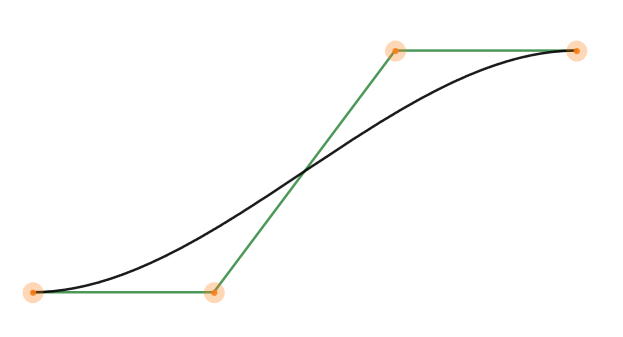
\includegraphics[width=0.8\textwidth]{graphics/bezier_curve.png}
        \caption{Bezier Curve}
	\end{figure}
This is implemented in our code as follows:
\begin{lstlisting}
// p[4] are the four anchor points
static SDL_Point BezierPoint(float t, SDL_Point p[4]){
    float tt = t * t;
    float ttt = tt * t;
    float u = 1 - t;
    float uu = u * u;
    float uuu = uu * u;

	//returns a point on the curve for a certain value of t
    return (SDL_Point){
       uuu * p[0].x + 3 * uu * t * p[1].x + 3 * u * tt * p[2].x + ttt * p[3].x,
       uuu * p[0].y + 3 * uu * t * p[1].y + 3 * u * tt * p[2].y + ttt * p[3].y};
}
/* Changing the value of t from 0 to 1 in 100 steps will give 100 points on the curve. We can draw lines between consecutive points to get the desired curve.*/
\end{lstlisting}
The above function only returns one point which lies on the curve. Curve cannot be drawn based on a single point. So the following function is called which calculates a bunch of points along the curve and joins them with lines to draw a curve:
\begin{lstlisting}
static void DrawWire(SDL_Point start, SDL_Point end, bool hilo, bool simulating){
    /*
        This function draws a 3px thick bezier curve (the wire) between points start and end
        this is done by drawing 3 bezier curves next to each other
        hilo boolean represents what signal the wire is carrying (high or low)
        simulating boolean represents whether simulation is running or not
    */
    SDL_Point wirePoints[MAX_WIRE_PTS]; // array of points which will be joined to make the wire
    for (int i = 0; i < 3; i++){
        // to align the starting and ending points
        if (abs(start.x - end.x) > abs(start.y - end.y)){
            start.y++;
            end.y++;
        }
        else{
            start.x++;
            end.x++;
        }
        // anchor points between start and end
        SDL_Point p2 = {start.x + (end.x - start.x) / 3, start.y};
        SDL_Point p3 = {end.x - (end.x - start.x) / 3, end.y};
        // setting color of the wire
        // set red color if hilo is true and simulation is running 
        // set blue color if hilo is false and simulation is running 
        // set green color simulation is not running 
        if (i == 1){
            // to give bezier curve in the middle a lighter color
            if (hilo && simulating)
                SDL_SetRenderDrawColor(renderer, HIGH_COLOR, 255);
            else if (!hilo && simulating)
                SDL_SetRenderDrawColor(renderer, LOW_COLOR, 255);
            else
                SDL_SetRenderDrawColor(renderer, WIRE_NEUTRAL, 255);
        }
        else{
            // to give bezier curve in the middle a darker color
            if (hilo && simulating)
                SDL_SetRenderDrawColor(renderer, WIRE_HIGH_D, 255);
            else if (!hilo && simulating)
                SDL_SetRenderDrawColor(renderer, WIRE_LOW_D, 255);
            else
                SDL_SetRenderDrawColor(renderer, WIRE_NEUTRAL_D, 255);
        }
        // calculate all points along the curve
        for (int i = 0; i < MAX_WIRE_PTS; i++){
            float t = (float)i / MAX_WIRE_PTS;
            wirePoints[i] = BezierPoint(t, (SDL_Point[4]){start, p2, p3, end});
        }
        // make sure that wire touches starting and ending points
        wirePoints[0] = start;
        wirePoints[MAX_WIRE_PTS - 1] = end;
        // join all the points with lines
        SDL_RenderDrawLines(renderer, wirePoints, MAX_WIRE_PTS);
    }
}
\end{lstlisting}
\end{document}
